% mnras
% \documentclass[fleqn,useAMS,usenatbib]{mnras}

% apj
%\documentclass[iop, twocolappendix, appendixfloats, numberedappendix, apj]{emulateapj}
%\documentclass[iop, twocolappendix, appendixfloats, numberedappendix, apj]{hackemulateapj}
%\documentclass{emulateapj}
\documentclass[twocolumn,twocolappendix,astrosym]{openjournal}

%=====================================================================
% CUSTOM: PACKAGES, MACROS & SETTINGS
%=====================================================================
% packages for figures
%\usepackage{graphicx,todonotes}
\usepackage{graphicx}

% packages for symbols
\usepackage{latexsym,amssymb}

% AMS-LaTeX package for e.g. subequations
\usepackage{amsmath,morefloats}
\usepackage[backref,breaklinks,colorlinks,citecolor=blue]{hyperref}
\usepackage{natbib,graphicx,amsmath,subfigure,color,xcolor}
\usepackage{verbatim}
\usepackage{threeparttable}

%\usepackage{natbib,graphicx,amsmath,subfigure,color,xcolor,hyperref}

\usepackage{pgfplots}
\pgfplotsset{compat=newest}
\usepgfplotslibrary{fillbetween}
\usepgfplotslibrary{groupplots}


%\usepackage{lineno}
%\linenumbers

\topmargin-1cm

\newcommand{\mrbtodo}[1]{\textcolor{red}{[MRB TODO: \bf #1]}}
\newcommand{\esstodo}[1]{\textcolor{orange}{[ESS TODO: \bf #1]}}

\newcommand{\descwl}{\texttt{WeakLensingDeblending}}

\newcommand{\vecg}{\mbox{\boldmath $g$}}
\newcommand{\vece}{\mbox{\boldmath $e$}}
\newcommand{\veck}{\mbox{\boldmath $k$}}
\newcommand{\vecQ}{\mbox{\boldmath $Q$}}
\newcommand{\vecF}{\mbox{\boldmath $F$}}
\newcommand{\vecD}{\mbox{\boldmath $D$}}
\newcommand{\vecc}{\mbox{\boldmath $c$}}
\newcommand{\vecm}{\mbox{\boldmath $m$}}
\newcommand{\matR}{\mbox{$\bf R$}}
\newcommand{\matC}{\mbox{$\bf C$}}
\newcommand{\bnab}{\boldsymbol{\nabla}}
\newcommand{\bnabg}{\boldsymbol{\nabla_g}}
\newcommand{\galsim}{\texttt{GALSIM}}
\newcommand{\ngmix}{\texttt{ngmix}}
\newcommand{\nnsim}{\texttt{nsim}}
\newcommand{\snr}{$S/N$}
\newcommand{\Tratio}{$T/T_{PSF}$}
\newcommand{\sn}{$S/N$}
\newcommand{\coadd}{{\rm coadd}}
\newcommand{\desreq}{$4\times 10^{-3}$}
\newcommand{\lsstreq}{$2\times 10^{-3}$}

\newcommand{\calexp}{\texttt{Exposure}}
\newcommand{\dm}{\texttt{LSST DM}}

\newcommand{\mcal}{\textsc{metacalibration}}
\newcommand{\mdet}{\textsc{metadetection}}
\newcommand{\Mcalshort}{\textsc{metacal}}
\newcommand{\Mcal}{\textsc{Metacalibration}}
\newcommand{\Mdet}{\textsc{Metadetection}}
\newcommand{\vest}{\mbox{\boldmath $e$}}
\newcommand{\est}{e}
\newcommand{\mcalR}{\mbox{\boldmath $R$}}
\newcommand{\mcalRS}{\mbox{\boldmath $R_S$}}
\newcommand{\gest}{\mbox{\boldmath $\hat \gamma$}}
\newcommand{\vecgam}{\mbox{\boldmath $\gamma$}}

\newcommand{\sx}{\textsc{Source Extractor}}

\newcommand{\bfd}{\textsc{BFD}}

\newcommand{\vonkarman}{{von K\'arm\'an}~}


%\setuphead[section][before={\testpage[2]}]

%mnras
%\title[\Mdet]{\Mdet: Mitigating Shear-dependent Object Detection Biases with \Mcal}

%\author[Sheldon et~al.]{Erin Sheldon$^1$, Matthew R. Becker$^2$,
%Niall MacCrann$^{3,4}$, Michael Jarvis$^5$
%  \\$^1$Brookhaven National Laboratory, Bldg. 510, Upton, NY 11973, USA
%  \\$^2$High Energy Physics Division, Argonne National Laboratory, Lemont, IL 60439, USA
%  \\$^3$Center for Cosmology and Astro-Particle Physics, The Ohio State University, Columbus, OH 43210, USA
%  \\$^4$Department of Physics, The Ohio State University, Columbus, OH 43210, USA
%  \\$^5$Department of Physics and Astronomy, University of Pennsylvania, Philadelphia, PA 19104, USA
%}


% apj
\shorttitle{Metadetection for Rubin}
\shortauthors{Sheldon, Becker, Jarvis, Armstrong}

\begin{document}
% mnrad
% \date{Draft \today}

% mnras
%\maketitle


% apj
%\title{\Mdet: Mitigating Shear-dependent Object Detection Biases with \Mcal}
\title{Metadetection for the Vera C. Rubin Observatory}

\author{Erin S. Sheldon}
\affil{Brookhaven National Laboratory, Bldg 510, Upton, New York 11973, USA}
\author{Matthew R. Becker}
\affil{High Energy Physics Division, Argonne National Laboratory, Lemont, IL 60439, USA}
\author{Michael Jarvis}
\affil{Department of Physics and Astronomy, University of Pennsylvania, Philadelphia, PA 19104, USA}
\author{Robert Armstrong}
\affil{Lawrence Livermore National Laboratory, Livermore, CA 94551, USA}


\begin{abstract}

        We present an implementation of the \mdet\ weak lensing shear
        measurement algorithm for use with the Rubin Observatory Legacy Survey
        of Space and Time (LSST).  This new code works with the data products
        produced by the LSST data management system (DM), and uses DM
        algorithms when possible.  We tested the code using a new set of
        simulations designed to mimic LSST imaging data.  The simulated images
        contain noise appropriate for LSST 10 year data, semi-realistic
        galaxies, and stars with representative distributions of magnitudes and
        spatial density.  Bright pixels were saturated and simulated bleed
        trails for bright stars were drawn when appropriate.  We also included
        bad columns and cosmic rays.  We interpolated all saturated features.
        Each image coordinate system was rotated randomly to mimic Rubin camera
        rotations.  The images had point spread functions (PSFs) with spatial
        variations expected for LSST.  The images were warped to a common frame
        and combined into overlapping coadd cells, excluding images with edges
        in the coadd region to retain a continuous point spread function.  We
        did not simulate the effects of inaccurate image calibration, PSF
        characterization, or artifact identification, but we did include simple
        background determination errors.  We turned on individual simulation
        features cumulatively in consecutive tests in order to isolate software
        bugs and possible biases.  The estimated shear was accurate within the
        expected LSST tolerances in all cases.  For our analysis choices, we
        found an effective galaxy density of $n_{\mathrm{eff}} \sim 41$ per
        square arcminute using the $r, i$ and $z$ band images for shear
        measurement.

        % Inadequate star masking can
        % lead to spurious object detections and problematic measurements that
        % would lead to significant additional noise, reducing the shear
        % sensitivity and $n_{\mathrm{eff}}$ significantly.  Given well
        % characterized input data, \mdet\ can provide accurate, high precision
        % shear measurements for LSST.

        % In this study we have demonstrated that, given well
        % characterized input data, \mdet\ can provide accurate, high precision
        % shear measurements for LSST.

\end{abstract}

% \newpage
% \tableofcontents

\section{Introduction} \label{sec:intro}

\esstodo{}

\section{Simulation Features} \label{sec:sim}

The basic simulation was similar to that created for \citep{mdet20}.  We added
additional features such as image artifacts, cosmic rays, stars, and saturated
stars which we will describe in the following sections.  All images were
rendered using the \galsim\ python package \citep{galsim2015}.

We simulated the calibrated exposure images produced by the LSST data
management system \citep[][\dm, version 0.2021.32]{JuricLSST2015,BoschHSC2017}.
This data is stored in an \calexp\ data structure, which carries a calibrated,
background subtracted image, along with an estimated noise variance image
plane, world coordinate system transformation (WCS) and position dependent PSF
model.  Problem areas associated with saturation, cosmic rays, and bad columns
are marked as separate bits in an integer bit mask image plane.

Other than background estimation errors (see \S \ref{sec:sim:bgerr}), we did not
test scenarios where the input data were mis-calibrated.  For example we did
not test the consequences of inaccurate PSF models, noise estimates or
photometric calibrations.  Our motivation was to test the performance of \mdet\
using well characterized data, or problems that could be addressed within
the shear code such as background errors.

For this work, we used the newly written simulation package
\texttt{descwl-shear-sims} version
0.4.2\footnote{\url{https://github.com/LSSTDESC/descwl-shear-sims}}.

\subsection{Image Filters and Noise} \label{sec:sim:noise}

We used the \descwl\ package
\citep{DESCWLSanchez2021}\footnote{\url{https://github.com/LSSTDESC/WeakLensingDeblending}}
to determine the noise for images in each filter.  In all simulation runs we
used predicted noise $n$ for the final 10 year coadd.  If $N$ simulated epochs
were used, we re-scaled the noise appropriately, such that the noise in each
epoch was $n * \sqrt{N}$.  We used a Guassian random field to simulate the
noise, which is a good approximation at the expected noise levels
\esstodo{cite}.

We did not add the expected amount of background to each image (but see \S
\ref{sec:sim:bgerr}).  After drawing all image features and adding
noise, we re-scaled the images to a common zero point of 30.

\subsection{Image World Coordinate System, Rotations and Dithers} \label{sec:sim:rotdith}

Each image was simulated as a tangent plane projection of the sky onto the
image frame with the LSST camera pixel scale of 0.2 arcseconds \esstodo{reference}.
The world coordinate system (WCS) transformation between sky and pixel
coordinates was represented as a \galsim\ \texttt{TanWCS} object.  Each
simulated WCS transformation had a random rotation applied, in order to mock up
the camera rotations used by LSSTCam \esstodo{cite proper paper}.  The center of
each image was shifted, or ``dithered'', randomly in two dimensions relative to
the center of the desired coadded image.  We choose the dithers to be a
unrealistically small, within two pixels, to minimize portions of the image
that would not overlap the final coadd.  We created images with size just large enough
so that the rotated image, after dithers, would have no edge crossing the coadd
region, again to avoid waste:  coadding an image with an edge produces a
discontinuous PSF in the final coadd, so such images would be discarded.

\subsection{Point Spread Function} \label{sec:sim:psfs}

For our basic PSF model we used a Moffat profile \citep{Moffat1969} with
shape parameter $\beta=2.5$ and full width at half maximum (FWHM) of 0.8 arcseconds.

We also generated spatially variable PSF models using the methods described in
Appendix~A of \citet{mdet20} based on work by \citet{heymans2012}.
\citet{heymans2012} used images with high stellar density to fit a \vonkarman\
model of atmospheric turbulence to the PSF variation. \citet{mdet20}
used this model, with a modification to reduce power below 1'', to generate
realizations of spatially variable PSFs using Gaussian random fields. The PSF
model is a Moffat \citep{Moffat1969} profile with shape parameter $\beta=2.5$
and variable size and shape. In \citet{mdet20} this approximate
variable PSF model was compared to detailed atmospheric and optics simulations.
It's parameters were set to generate the typical spatial PSF variance expected
expects for Rubin exposures. The median FWHM of the generated PSFs was 0.8
arcseconds.  We also ran simulations with larger than expected variations in
order to test the accuracy of the PSF coadd under extreme conditions.

\subsection{Stars} \label{sec:sim:stars}

We simulated stars using fluxes and densities sampled from the LSST DESC DC2
simulation \esstodo{cite}.  For each simulated field we sampled randomly, with
replacement, from the map of stellar density used to generate DC2, rejecting
densities higher than 100 per square arcminute.  This density represents
the total number of stars drawn, not the number detected.  We
sampled the multiband flux the DC2 star catalog.  We modeled
each star as a small Gaussian (FWHM $= 10^{-4}$ arcsec) convolved with the
point spread function.  We drew stars at random locations, even when galaxies
were drawn on a grid layout (see \S \ref{sec:sim:layouts}).  Stars were allowed
to saturate and have an associated bleed trail (see
\S \ref{sec:sim:satbleeds}).

\subsection{Image Saturation, Star Masking and Star Bleed Trails} \label{sec:sim:satbleeds}

The value in each pixel was artificially limited in order to simulate
saturation, and saturated pixels were marked with an appropriate flag in the
integer bitmask image of the \calexp, and the variance for those
pixels was set to infinity.  Non linear detector response was not simulated.

Saturated stars were over-drawn with a simulated bleed trail image, taken from
a set of previously generated templates.  The bleed templates were identified
in images of bright stars created using the DC2 code.  For each saturated star
in our simulation, we found a close template match in the filter of interest
and drew the associated bleed image directly over the star image with a value
set to the saturation level. The bleed pixels were marked with the appropriate
flag in the bitmask.

We further masked saturated stars a circular mask that covered the star out to
the radius where the profile reached the noise level.  Note in real data such a
mask would need to be determined algorithmically.   This region was set to zero
in the image and marked appropriately in the bitmask.   This mask does not
necessarily cover the bleed trail completely, although the trail was
interpolated (see \S \ref{sec:coadding}).  We find that these unmasked trails
do not cause a shear bias, which we attribute to the camera rotations that
randomize the direction of the trail on the sky.

Masks with sharp features can cause ringing in the FFTs used by the \mdet\
algorithm.   Each star mask is like a circular ``tophat'', which will have a
sharp feature where it intersects an object in the image.  We mitigated this
effect using the apodization procedure described in \citet{BeckerMdetCoadd}. We
extended the star mask by 16 pixels and forced the mask to smoothly transition
from zero in the interior of the circle to unity at the expanded edge. The
transition region was parameterized using the cumulative integral of a
triweight kernel. This kernel is a function of two parameters, $m$ and $h$, and
is defined for a point $x$ with quantity $y = (x-m)/h$ as
\begin{equation}
K(x, m, h) = \begin{cases}
0 & y < -3 \\
(-5y^7 / 69984 \\
+ 7y^5 / 2592 \\
- 35y^3 / 864 & -3 \le y \le 3 \\
+ 35y / 96 \\
+ 1 / 2) \\
1 & y > 3
\end{cases}
\end{equation}
The kernel goes from zero to unity over a span of $6h$, centered on $m$.
The general logic is to set $h$ large enough that the variation across the edge is slower
than the variation given by the PSF profile, but not so large that area in the image is
wasted. We set $h$ to 1.5 pixels and set $m$ to the radius of the star mask hole.

\subsection{Cosmic Rays \& Bad Columns} \label{sec:sim:cosmics_badcols}

We followed \citet{BeckerMdetCoadd} in generating bad column and cosmic ray artifacts.
For cosmic rays, we selected a random location on the image, a random angle, and a random
length between 10 and 30 pixels. We then flagged pixels along this line as having been hit
by a cosmic ray, making sure that pixels that touch only along corners have the pixels
directly adjacent to them flagged as well. We set a cosmic ray bit in the bitmask for
interpolation later and set the image value to \texttt{NaN} to ensure that no flagged
pixels are inadvertently used in the final shear estimates.

We generated bad column masks using a slightly modified Monte Carlo generator
from \citet{BeckerMdetCoadd}. Each bad column was a single pixel wide,
positioned randomly on the image. We also added gaps at random to the bad
columns to simulate bad columns which do not span the full CCD.  We generated
a single bad column for each image.

The LSST lensing analysis will be carried out on coadd images of hundreds of
exposures, with artifacts interpolated on the original data before being warped
and added.  The aggregate number of artifacts will be large, but the impact of
each artifact will be relatively small.  It was not computationally feasible to
simulate such a large number of epochs in order to test the effect of artifacts
in a realistic way.  Rather we simulated a smaller number of epochs per
band, typically
1 but up to 10, with the noise scaled so that the final coadd noise matched
LSST 10 year data.  Thus, relative to expected LSST data the impact of each
artifact on the coadd was large but the aggregate number of artifacts was
small.

\subsection{Galaxies} \label{sec:sim:galaxies}

We used the \descwl\ package to generate galaxy models \esstodo{cite}.  These
elliptical, color models have bulge, disk and AGN components.  Rather than use
the \descwl\ package to draw the models in the image, we drew the models in our
code in order to enable the use of our own PSF models (see \S
\ref{sec:sim:psfs}), and to allow for more efficient drawing.

We also performed simulation runs with single component, round exponential
galaxies with fixed flux and size.  These models are useful for shear recovery
tests that do not require a realistic galaxy population, but benefit from using
low shape noise shear tracers.  These models were also used for moderately
fast, full shear recovery tests, to further verify code changes that had
already passed the faster unit tests.

\subsection{Layouts} \label{sec:sim:layouts}

We ran tests with both random and gridded galaxy layouts.  The random layout
was used with the realistic galaxy population, with a density of objects that
reflected the expected density of galaxies as defined in the \descwl\ package.
The grid was used with the simple, round exponential galaxies to facilitate
moderately fast shear recovery tests.  The grid was square, with spacing
designed to avoid overlap between adjacent galaxies, and thus avoid blending
effects.

See \S \ref{sec:sim:galaxies} for descriptions of each galaxy model type.

\subsection{Image Background} \label{sec:sim:bgerr}

We add a negative constant to the images to approximate errors in the
background determination.  The motivation is to test if errors for individual
epochs can be corrected in the final coadd image by running a second background
determination.

\subsection{Shear Patterns} \label{sec:sim:shears}

We implemented two different types of shear pattern.  In one we used a single
shear for all images, with constant magnitude and orientation.  The second type
was a constant magnitude shear, but with random orientation for each image.
These two scenarios result in equivalent shear recovery bias when objects are
not divided into cells on the sky (see \S \ref{sec:sim:cells}) but, as we will
see in \S \ref{sec:results:cells}, a small additional selection bias is
introduced for random shears when when trimming to cells.

\subsection{Overlapping Coadd Cells} \label{sec:sim:cells}

Coadds can be used for shear measurement\citep{ArmstrongCoadd}, but we
require that the coadded images have a continuous PSF in order to faciliate
accurate PSF modeling.  Images that have an edge in the coadd region must be
rejected.  Smaller coadds result in fewer images being rejected, but very small
coadds would complicate object identification and deblending.  For LSST, we plan to
use relatively small (250x250 pixels) overlapping (50 pixels) coadded regions
for shear measurement, which we call ``cells'' \esstodo{cite} because they
are small subregions of the larger ``tract'' regions defined within the
\dm\ framework.

We ran simulations with and without cells in order control for issues specific
to the cell processing and trimming of objects to non overlapping regions.  We
adopted the cell definitions outlined above: 250x250 pixel cells with 50 pixel
overlaps. The object list was trimmed to the non-overlapping region in post
processing.

\subsection{Noise Images} \label{sec:sim:noiseimages}

The \mcal\ procedure involves deconvolution by the PSF, shearing of the image,
and reconvolution by a round kernel.  This process alters the noise and
produces a spurious shear response \citep{SheldonMcal2017}.  We can cancel this
bias by adding a noise image, with properties that statistically match the real
background noise, processed in a similar manner but with orthogonal shear
\citep{SheldonMcal2017,mdet20}.  We stored this noise image in a copy of the image
\calexp\ structure, but replacing the real image data with the noise image.

\begin{figure}
    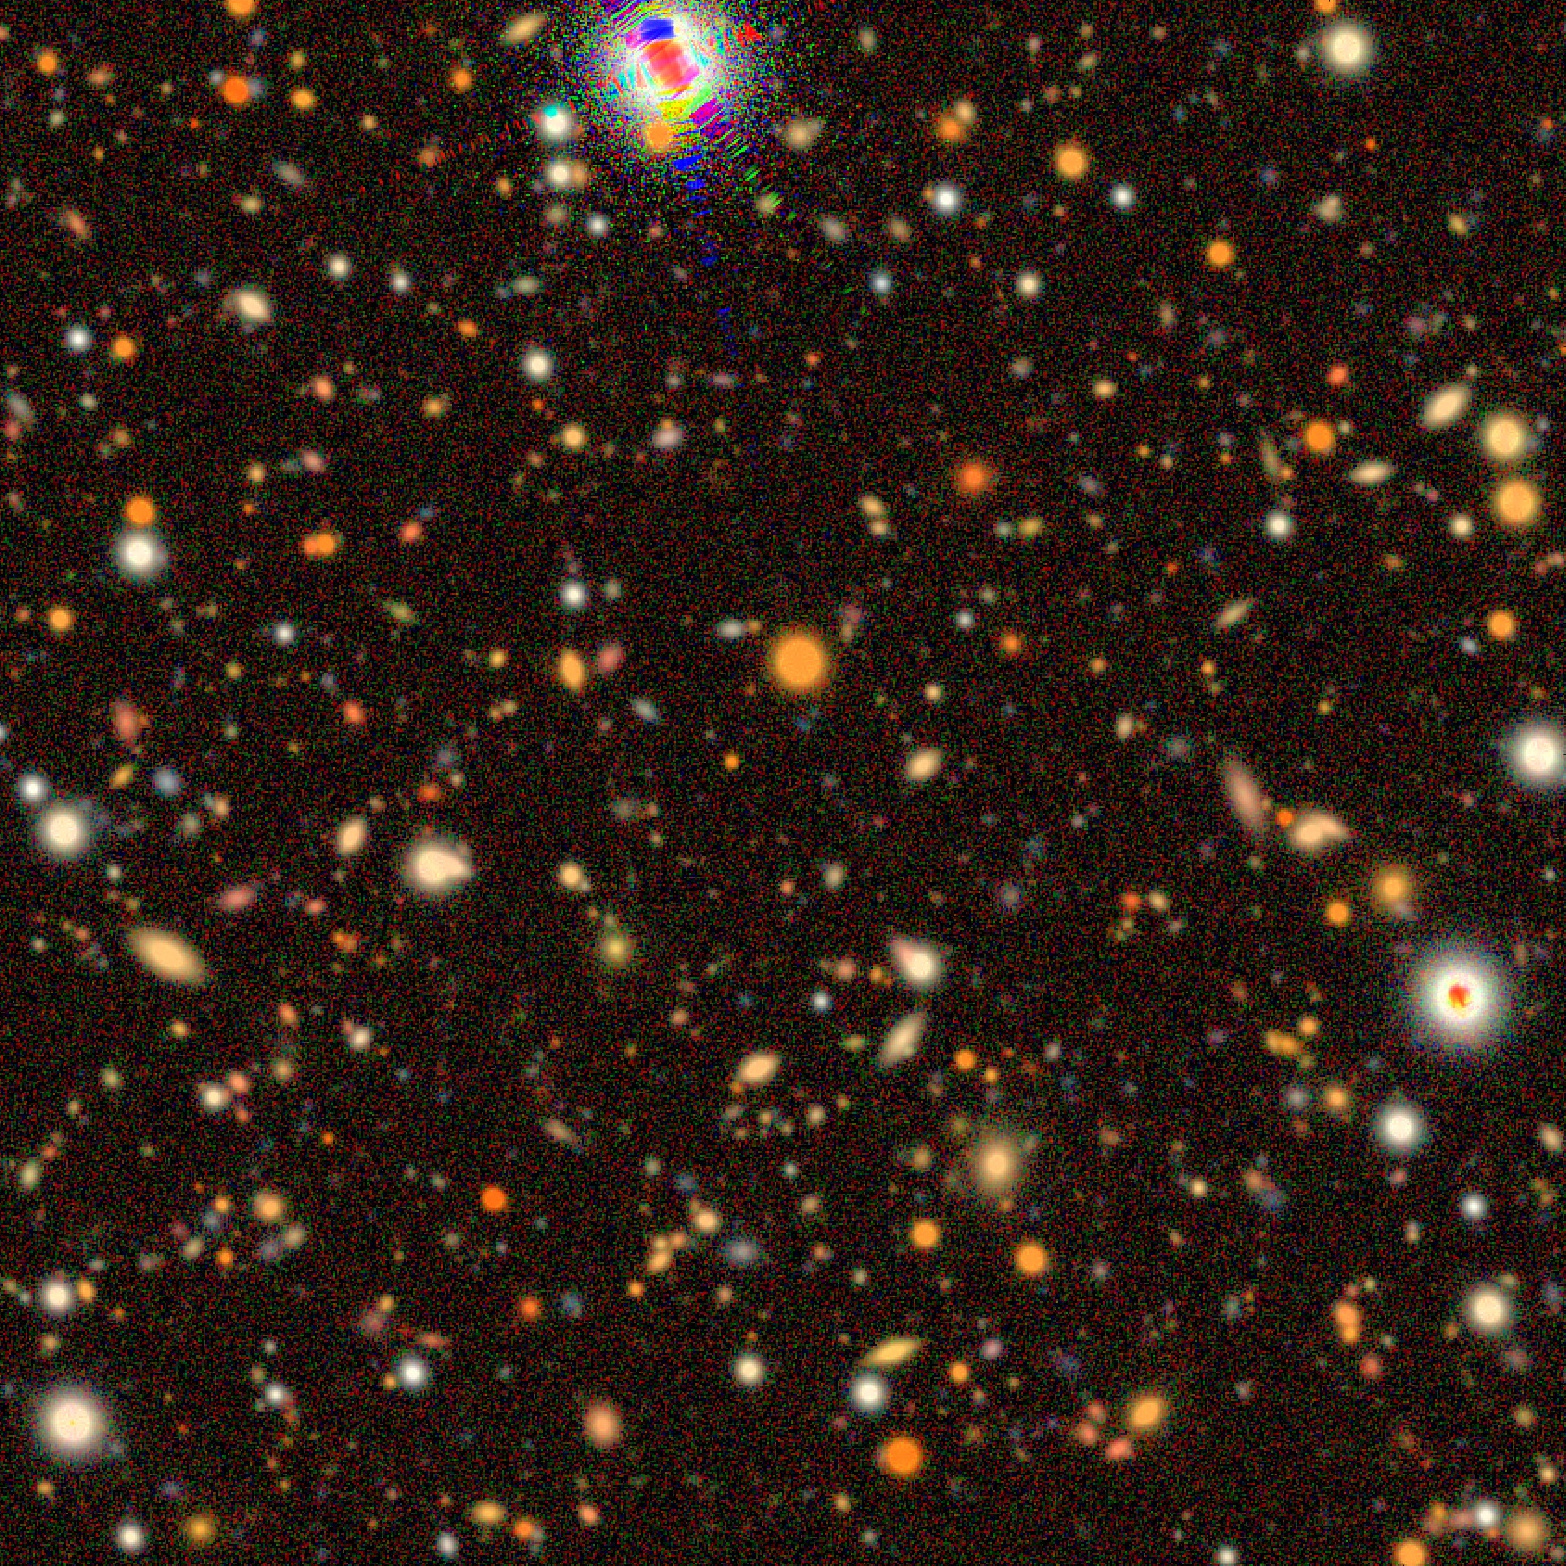
\includegraphics[width=\columnwidth]{example-image.jpg}
    \caption{
        Example simulated image using one ``epoch'' for each of the $r$, $i$,
        and $z$ bands, with noise corresponding to the 10 LSST coadd data.
        The images have been warped and coadded, although in this case there
        is but a single warped image.
        Note the interpolated bleed trails around a bright star in the upper
        part of the image, appearing at different orientations due to the
        simulated camera rotations.
    } \label{fig:colorimage}
\end{figure}
\begin{figure}
    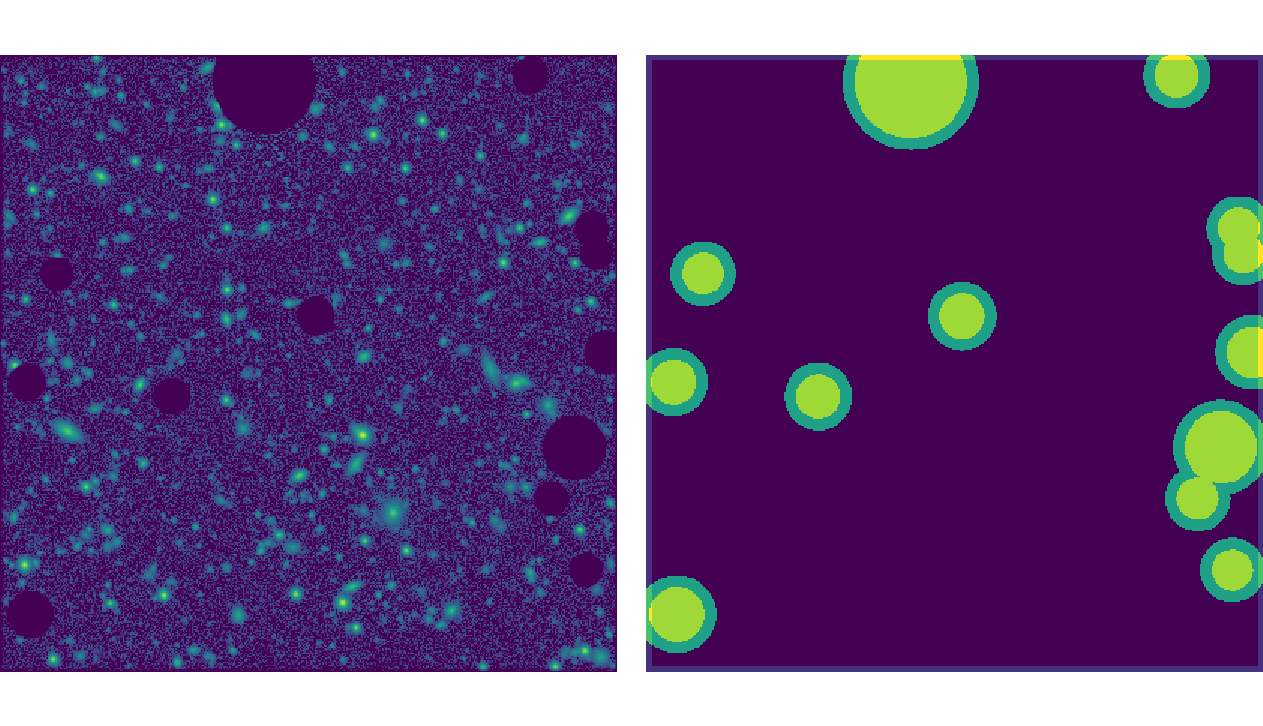
\includegraphics[width=\columnwidth]{example-masked-image.pdf}
    \caption{
        Example masked images, corresponding to the images in figure
        \ref{fig:colorimage}.  The rows correspond to $r, i$, and $z$ bands
        respectively.  The left column shows the masked image, the middle the
        noise variance, and the right the bitmask plane.  The circles show the
        star masks applied to each type of image, which are retained in the
        coadd bitmask to facilitate processing near stars.  In the original
        images, there are also pixels marked for cosmic rays and bad
        columns, but these are not retained in the coadd bitmask.
    }
\end{figure}



\section{Image and PSF Coaddition} \label{sec:coadding}

For coaddition, we used the package \texttt{descwl\_coadd} version
0.3.0\footnote{\url{https://github.com/LSSTDESC/descwl_coadd}}.  This code uses
\dm\ algorithms for warping images onto the coadd pixel grid, in particular the
\texttt{AccumulatorMeanStack} from \texttt{lsst.meas.algorithms} sub package.
We used an inverse variance weighting, based on the noise in the image.

Before warping, we interpolated the simulated artifacts in each image such as
cosmic rays, bad columns, and saturated pixels.  The interpolation and warping
modifies the noise properties of the image.  Thus, for accurate \mcal\ noise
corrections (see \S \ref{sec:sim:noiseimages}) we must also run the noise image
through the same procedures.

Rather than use the \dm\ interpolation codes, we performed all
interpolation of artifacts and saturated regions using the
\texttt{CloughTocher2DInterpolator} from the scipy software
package\footnote{\url{https://docs.scipy.org/doc/scipy/reference/generated/scipy.interpolate.CloughTocher2DInterpolator.html}}.
We used this interpolation because the \dm\ cosmic ray interpolation available
at the time of writing is intertwined with the detection of cosmic rays, so
cannot be run on the noise image.

Using the same code, we also created PSF coadded images.  For each input image,
we generated an image of the PSF at the location of the coadd center, including
any sub-pixel offsets between the pixel grids, so the PSF images where
generally not centered.  We then warped these and coadded these images using
the same weights as the image data.  The off-centering and warping is important
so that the PSF includes the same small amount of smearing present in the image
interpolation.  Not including this offset results in percent level
multiplicative shear biases \citep{ArmstrongCoadd}.  Note \dm\ provides a
PSF coadding code, but at the time of writing it did not perform sub-pixel
offsets, so was unsuitable for our purposes.

The resulting coadd and PSF coadd data were stored in a new \calexp\ data
structure for use in \mdet.

\section{Metadetection} \label{sec:mdet}

For shear inference we used the \mdet\ method presented in \cite{mdet20}.
\Mdet\ is an extension of the \mcal\ method
\citep{HuffMcal2017,SheldonMcal2017} to include the object identification
stage. We call this ``detection'', meaning specifically object identification
rather than detection of pixels with significant signal.  \Mdet\ mitigates
biases due to the shear-dependent nature of the detection processing in finite
resolution images, biases which are expected to be a few percent for LSST
\citep{mdet20}.

Briefly, with \cal\ we assume that the true applied, two-component shear
$\boldsymbol{\gamma}$ is small, so that a measured ellipticity $\boldsymbol{e}$
of a galaxy is linear in the shear:
\begin{eqnarray} \label{eq:response}
\boldsymbol{e} & \approx & \left.\boldsymbol{e}\right|_{\gamma=0} +
                           \left.\frac{\partial \boldsymbol{e}}{\partial\boldsymbol\gamma}\right|_{\gamma=0} \boldsymbol\gamma +
                           O(\boldsymbol\gamma^2)\nonumber\\
               & \equiv  & \left.\boldsymbol{e}\right|_{\gamma=0} +
                           \boldsymbol{R} \boldsymbol\gamma +
                           O(\boldsymbol\gamma^2)
\end{eqnarray}
Here, the matrix $\boldsymbol{R}$ represents the linear response of the
measurement to an applied shear. It can be written component wise as
$R_{ij}=\partial e_i /\partial \gamma_j$, with $i$ and
$j$ taking all combinations of the two shear components.  For ellipticity
measurements we use weighted moments (see \S \ref{sec:mdet:meas}).

We use a finite difference to estimate $\boldsymbol{R}$.  The image is
deconvolved by the PSF, sheared, and reconvolved with a round kernel.  This
process is repeated for a small positive and negative shear, and a finite
difference response term is formed
\begin{equation}
R_{ij} \approx \frac{e_i^{+} - e_i^{-}}{\Delta\gamma_j}\ .
\end{equation}
where $e_i^{+}$ is measured on the positively sheared image and $e_i^{-}$ is
measured on the negatively sheared image.

As mentioned in \S \ref{sec:sim:noiseimages}, the deconvolve, shear, reconvolve
process produces a spurious shear response that we correct by adding a noise
image run through the same process but with orthogonal shear.

The responses are too noisy to be applied to individual ellipticity measurements.
We instead average the shapes and responses in equation \ref{eq:response} to
recover a mean shear \vecg
\begin{eqnarray} \label{eq:shearmeas}
    \left< \boldsymbol{R} \right> &=& \left< \frac{\partial \boldsymbol{e} }{\partial \boldsymbol{\gamma} } \biggr\rvert_{\gamma=0} \right>, \nonumber \\
    \langle R_{ij}\rangle &=& \left< \frac{e_i^{+} - e_i^{-}}{\Delta\gamma_j} \right>, \nonumber \\
    \langle \vecg \rangle & \approx & \langle \boldsymbol{R}\rangle^{-1}\langle\boldsymbol{e}\rangle.
\end{eqnarray}

However, this process is incomplete:  the detection phase also depends on
shear.  We can incorporate detection by running object detection on the image
as well as the sheared images independently and producing the averages from
separate catalogs.  Moving the derivative outside of the average, we find
\begin{eqnarray} \label{eq:fullR}
    \left< \boldsymbol{R} \right> &=& \frac{\partial \left< \boldsymbol{e} \right> }{\partial \boldsymbol{\gamma} } \biggr\rvert_{\gamma=0},  \nonumber \\
    \langle R_{ij}\rangle &=& \frac{\langle e_i^{+}\rangle - \langle e_i^{-}\rangle}{\Delta\gamma_j} \nonumber \\
\end{eqnarray}
where now the averages for $e_i^{+/-}$ are for object catalogs found on the
respective ${+/-}$ sheared image.

For \mdet, we used the package \texttt{metadetect} version
0.8.2\footnote{\url{https://github.com/esheldon/mdetadetect}}.  In the following subsections
we will describe parts of this process in more detail.

\subsection{Creation of Sheared Images} \label{sec:mdet:sheared}

For this work we used \dm\ data structures to represent image data (see \S
\ref{sec:sim}).  We adapted the \mcal\ implementation for creating sheared
images from the \texttt{ngmix}
package\footnote{\url{https://github.com/esheldon/ngmix}} to use these data
structures.  The new code is part of the \texttt{metadetect} software package.


\subsection{Detection and Deblending} \label{sec:mdet:detect}

We used the \dm\ algorithm for detection \esstodo{cite Jims paper}.  We ran with
the default settings at the time of writing, which retains sources with a
$S/N \gtrsim 5$ calculated from a PSF template flux measurement.  Before detection
we re-determined the background to remove the background estimation errors that were
put into the simulation (see \S \ref{sec:sim:bgerr}).

Deblending was performed during the object detection phase as part of the
process of finding sub-peaks, but we did not use the deblender to remove the
light of neighboring objects when measuring object properties (see \S
\ref{sec:mdet:meas}).  We found that using the models to remove neighbor light
resulted in shear biases of order ten percent.

We did limited testing with the Scarlet \esstodo{cite} deblender, which has
recently received support in the \dm\ software stack. Scarlet performed better
in the limited tests we performed, but due to the high computational cost of
the deblender, we did not gather enough statistics to perform comprehensive
tests.

As we will show in \S \ref{sec:results}, measuring shapes without deblending
the light of neighbors caused no detectable bias.  However, deblending may
improve the accuracy of other critical tasks such as inferring the redshift
distribution of the lensing source galaxies.  We will explore deblending more
in future work.

\subsection{Object Measurement} \label{sec:mdet:meas}

We used version v2.1.0 of the \ngmix\ package to measure weighted moments for
each detected object. The weight function was a fixed, circular, Gaussian $G(x,
y)$ with FWHM=1.2 arcseconds.  We recorded the flux,
S/N, second moments, and ellipticity derived from the second moments:
\begin{eqnarray} \label{eq:moments}
    F &=& \sum G(x, y) I(x, y) \nonumber \\
    \sigma^2(F) &=& \sum G(x, y)^2 \sigma^2(I(x, y)) \nonumber \\
    T &=& \sum G(x, y) I(x, y) ~ (x^2 + y^2) \nonumber \\
    M_1 &=& \sum G(x, y) I(x, y) ~ (x^2 - y^2) \\
    M_2 &=& \sum G(x, y) I(x, y) ~ 2 x y \nonumber \\
    e_1 &=& M_1 / T \nonumber \\
    e_2 &=& M_2 / T \nonumber \\
    S/N &=& F / \sigma(F) \nonumber
\end{eqnarray}
where $I(x, y)$ is the intensity of the image, and $\sigma^2(I(x, y))$ is the
noise variance. The sums run over all pixels in a 48x48 postage stamp image
extracted around the object of interest.  The $x$ and $y$ coordinates are
relative to the center found during detection.  Not shown in the sums is the
weight for each pixel in the sum, which is the inverse of the pixel noise
variance. However, the noise variance is nearly constant across the coadd so
this is only relevant for masked, zero weight pixels.  Note $T$ is an estimate
of the observed square size of the object, not the pre-PSF size.
We also calculated variances for the moments and ellipticities.

We also record the moments of the coadded PSF for use in object selection (see
\S \ref{sec:results:full}).


\section{Running the Simulation and Metadetection} \label{sec:running}

We used the ``wrapper'' package \texttt{mdet-lsst-sim} version
0.3.4\footnote{\url{https://github.com/esheldon/mdet-lsst-sim}} to run the
simulation, coaddition and \mdet, and to organize, submit and collate large
runs on computing clusters.

In all cases we used a constant shear, with possible random shear orientations
for each simulated scene (see \S \ref{sec:sim:shears}).  We simulated each
scene twice, with equal but opposite shears, in order to implement the noise
canceling method of \cite{pujol2019}.  For randomized shear directions, the
shape measurements from different scenes where placed in a common reference
frame before averaging to get a mean shear.

We estimated the uncertainty in the averaged shear measurements using a
jackknife technique (\esstodo{cite}), with chunks defined as a few tens to hundreds of scenes.
The jackknife technique gives a significantly larger uncertainty than a
straight error propagation using the shape noise due to extra sources of error
associated with masking, deblending, stellar contamination and variable
response.

\section{Results} \label{sec:results}

In this section we present the results for various simulation and analysis
configurations.

We identify our ``base'' simulation as one with fixed size, high S/N, round
galaxies on a grid layout, which provides the highest signal-to-noise ratio for
the shear recovery. From the results in \citet{mdet20}, we expect a small bias
in this configuration due to higher order shear effects (see \S
\ref{sec:results:base}).

We performed shear recovery turning on each feature successively in order to
isolate the cause of potential biases.  We found a bias only in the case of
extreme spatial PSF variation with few simulated epochs (see \S
\ref{sec:results:psfvar}).  We present results including all simulation
features in \S \ref{sec:results:cells}.

To characterize the bias, we assume a simple linear model \citep[see,
e.g.,][]{heymans2006} for estimating a bias in the recovered shear
\begin{equation} \label{eq:m}
\vecg = \vecc + (1 + \vecm) \vecgam
\end{equation}
where \vecg\ is the inferred shear, measured using equation \ref{eq:shearmeas},
\vecgam\ is the true shear, \vecc\ is the additive bias, and \vecm\ is the
multiplicative bias. We found \vecc\ was consistent with zero in all tests, so
in what follows we only report \vecm.

\subsection{Baseline Results for Fixed Galaxies on a Grid} \label{sec:results:base}

In order to establish a baseline for the bias due to higher order shear
effects, we ran a simulation with fixed, round exponential, S/N $= 10,000$,
half light radius 0.5 arcsecond galaxies placed in the grid layout (see
sections \ref{sec:sim:galaxies} and \ref{sec:sim:layouts}) with image dithers
and rotations.  In order to make the test as efficient as possible, we used
only the $i$ band with a single image ``epoch''.  We used a fixed Moffat
PSF\citep{Moffat1969} with FWHM=0.8.  We expect a bias $m$ of a few parts in
ten thousand for this sim \citep{SheldonMcal2017}.  We found a bias of
$4.2\times 10^{-4} < m < 4.3\times 10^{-4}$ (99.7\%~confidence), consistent
with our expectations.

We reran this simulation after all major code updates as a kind of extended
unit test to expose bugs and regressions.

\subsection{PSF Variation} \label{sec:results:psfvar}

In order to measure the shear response, the \mdet\ algorithm creates
artificially sheared versions of each coadd image (see \S \ref{sec:mdet}).
This process involves deconvolving the image by the PSF (see \S
\ref{sec:mdet}).  This deconvolution would require a spatially dependent kernel
for spatially varying PSFs.  However, due to the camera rotations, and large
number of images used to make the coadd, we expect the variation in the final
image to be significantly reduced.  Thus the single coadded PSF that we
generate at the coadd center (see \S \ref{sec:sim:psfs}) may be sufficient.

We ran the same grid simulation from \S \ref{sec:results:base} with the
spatially varying PSF presented in \S \ref{sec:sim:psfs}. We used the $r, i, z$
bands but with a single image epoch per band, with rotations and dithers.  We
did not see any increase in the bias.   We interpret this result to indicate
that the PSF variation is small enough that our single coadded PSF is
sufficient, even with a single image per band.

We also ran with the same simulation configuration, but with ten times the
expected PSF variation. In this case, for a single image per band, we found a
small increase in the bias $m \sim 0.0016$.  However, after increasing the
number of simulated epochs per band to ten but with the same final coadd noise
level, we no longer found this extra bias.  We interpret this to mean that more
epochs are required to cancel out very large PSF variations.  LSST will take
hundreds of images in each band (\esstodo{cite}), so we do no expect PSF
variation to be a significant source of bias.

For the remaining tests in this paper we use a spatially variable PSF with
expected level of variation.

\subsection{Results with Additional Simulation Features} \label{sec:results:more}

We ran the simulation with realistic galaxies, random layout, image
artifacts, and background subtraction errors, as listed in \S \ref{sec:sim}.

For the realistic galaxy configuration, we adopted a basic set of cuts
\begin{eqnarray} \label{eq:basiccuts}
    \mathrm{S/N} & > & 12.5 \\
    T/T_{PSF} & > & 1.2
\end{eqnarray}
where $T$ is the Gaussian weighted square size of the observed, PSF convolved
image, as defined in equation \ref{eq:moments}, and $T_{PSF}$ is the
corresponding value for the PSF.  The lower \snr\ cut is motivated by the noise
study in \S \ref{sec:results:sdensnoise} in which a cut at 10 or 12.5 resulted
in similar shear uncertainties.  In all the following tests, using a lower
bound of $S/N > 10$ gave consistent results.

The lower cut on $T/T_{PSF}$ represents a simple attempt to remove stars from
the sample.  For \mcal, including stars in the sample does not result in a
biased shear when the PSF is accurately modeled \citep{SheldonMcal2017}.  With
\mdet\ the stars may result in a small bias because their positions are not
moved by the true shear, but {\it are} moved by the artificial shear. However,
the bias caused by this counterfactual movement is small \citep{mdet20}.
Nevertheless, it may be desirable to remove stars for other reasons, such as to
avoid confusion when determining the redshift distribution, so we include a
crude star removal in our tests.

We again turned on each feature successively in order to isolate possible
biases.  In no case did we find additional bias in the shear recovery beyond
that expected from higher order shear effects (see \S \ref{sec:results:base}).
More details are given in the following sub-sections.

\subsubsection{Results with Varied Selections on Object Properties} \label{sec:results:select}

We varied the selections on object size ratio $T/T_{PSF}$ and \snr\ and
repeated the shear recovery analysis.  The results are shown in figure
\ref{fig:trends}, for both constant and spatially varying PSFs (see \S
\ref{sec:sim:psfs}).  We did not detect any additional bias.  Note that
stricter cuts on \snr\ resulted in lower noise for this test because the noise
cancellation procedure which works better for bright objects.  We will explore
the shear sensitivity without noise cancellation in \S
\ref{sec:results:sdensnoise}.

\begin{figure}
	\includegraphics[width=\columnwidth]{{trends}.pdf}

    \caption{Multiplicative shear bias $m$ for a simulation with a realistic
    galaxy sample, random galaxy layout, image artifacts and background
    subtraction errors.  The top panel shows the bias as a function of \snr\
    and the bottom panel shows the bias as a function of the size ratio
    \Tratio.  The dot-dashed line represents the approximate expected bias due
    to higher order shear effects, and the solid shaded band represents our
    nominal accuracy goal.  The hatched areas show the 99.7\%~confidence bands
    for the constant PSF (hatched) and spatially variable PSF (solid).  In all
    cases the results are consistent with the expected bias.}
    \label{fig:trends}

\end{figure}

\subsection{Results with Overlapping Coadd Cells} \label{sec:results:cells}

We ran a modification of the base simulation as described in \S
\ref{sec:results:base} with a randomized position layout and overlapping cells
as described in \S \ref{sec:sim:cells}.  Because the cells overlap, the catalog
created for each coadd must be trimmed to a unique region.  Shear changes the
locations of objects, so this trimming introduces a shear dependent selection
effect.  For \mdet\ to correct for this selection, it is important that the
full scene be sheared, so that the object positions change after application of
the counterfactual shear.  Using unsheared positions can result multiplicative
biases of a few tenths of a percent.

In the case where the true simulated shear aligns with the artificially applied
shear used to create the \mcal\ images, we found that \mdet\ provided an
accurate calibration.  However, when using randomized shear orientations (see
\S \ref{sec:sim:shears}), we found the multiplicative bias $m$ was below the
expected bias due to higher order shear effects by about $-0.0004$.  Our
interpretation is that the artificial shearing slightly over-predicts the
selection effect when it is not perfectly aligned with the true shear.  This
bias is smaller than LSST requirements $|m| \lesssim 0.001$.  Nevertheless, we
speculate that using artificial shears with random orientations could mitigate
this effect.  We may explore this more in a future work.

\subsection{Results with Stars and Bleed Trails} \label{sec:results:full}

Our ``full'' simulation configuration included stars and bleed trails as
described in \S \ref{sec:sim:stars} and \ref{sec:sim:satbleeds}, in addition to
the features tested in the previous sections.  We discuss aspects of the
measurements and results below.

\subsubsection{Weighting}

For the full simulation configuration we found it beneficial to apply weights
in the shear average.  We used a two part weight function
\begin{equation}
    W(\sigma_g, g) = W_\sigma (\sigma_g) \times W_g(g)
\end{equation}
with $W_\sigma$ based on the object's shape noise and $W_g$ designed to
down-weight a particular set of spurious objects.

The primary weight was based on the intrinsic shape noise and shape
measurement uncertainty, and is designed to be an optimal weight in the
scenario that the only sources of uncertainty are the intrinsic shape noise 
and shot noise in the images
\begin{equation}
    W_\sigma = \frac{1}{\sigma_{SN}^2 + \sigma_g^2},
\end{equation}
\esstodo{cite}
where $\sigma_{SN}$ is the intrinsic ellipticity noise of the population and
$\sigma_g$ is the estimated uncertainty from shot noise.  We find $\sigma_{SN}$
before response correction is about 0.07.  The average response is about 0.24
for this sample, implying the true shape noise is about 0.29.

In the presence of stars we found an unexpected population of high ellipticity
objects.  These objects were usually spurious detections or blends of faint
objects with bright stars, found just outside the star masking radius
discuessed in \S \ref{sec:sim:satbleeds}\footnote{Masaya Yamamoto, private
communication}.  We did not keep enough information in the output files to
exclude these objects from our catalogs in post processing, and rerunning was
would have taken prohibitively long due to limited computing resources.  As a
temporary solution we included an additional ellipticity dependent weight
function \citep{ba14}
\begin{equation}
    W_g(g) = \left[1 - g^2\right]^2 \mathrm{exp}\left[ -g^2/2 \sigma_w^2\right]
\end{equation}
where $g$ is the total scalar shape $g = \sqrt{g_1^2 + g_2^2}$.  We took
$\sigma_w = 0.3$, which downweights very high ellipticity objects.  We found
that using this weight function reduced the uncertainty of the shear recovery
by 13\%.  In future work it will be important to use sufficient star masking,
and identify problematic objects.

\subsubsection{Dependence of Shear Bias on Stellar Density Cut} \label{sec:results:sdens}

In figure \ref{fig:stardens} we show the multiplicative bias as a function of
maximum stellar density and various cuts on the measured signal to noise ratio,
in addition to a common cut on size ratio $T/T_{PSF} > 1.2$.  In no case did we
detect a bias beyond that expected from higher order shear effects.

\begin{figure}
	\includegraphics[width=\columnwidth]{{stardens-bias}.pdf}

	\caption{
        Multiplicative bias $m$ as a function of maximum stellar density cut
        for various cuts on \snr. The hatched areas show the 99.7\%~confidence bands
        for the various cuts.  The dot-dashed line represents the
        approximate expected bias due to higher order shear effects, the
        solid shaded band represent our nominal accuracy goal.  In no case did we
        detect any bias beyond expectations.
    } \label{fig:stardens}

\end{figure}

\subsubsection{Dependence of Shear Sensitivity on Object Selections}
\label{sec:results:sdensnoise}

We explored the dependence of the shear sensitivity on stellar density and
\snr.  In order to get an accurate measure of the relative uncertainty, we did
not cancel noise using the results from paired images.  The noise cancellation
is most effective for higher \snr\ objects that are more likely to be detected
in both of the paired images, so using it would result in artificially smaller
uncertainties for higher minimum \snr\ cuts.

In figure \ref{fig:stardenserror} we show the uncertainty in the recovered
shear as a function of maximum allowed stellar density and \snr\ cut, relative
to the cuts that provide the lowest noise.

We find the uncertainty decreases with the maximum allowed stellar density. The
dependence on stellar density is fairly flat at high stellar density.
Including higher stellar density areas reduces the noise, but with limited
benefit beyond a density of about 40 stars per square arcminute.  A relatively
small fraction of the simulated area has high stellar density, and fields with
high stellar density tend to have a relatively large area masked due to stars.

\begin{figure}
    \includegraphics[width=\columnwidth]{{stardens-nocancel-error}.pdf}

    \caption{Shear measurement sensitivity as a function of maximum stellar
    density and cuts on various measured object properties, relative to the
    cuts that give the best sensitivity.  We find that less restrictive cuts on
    stellar density result in lower sensitivity, but with marginal improvement
    beyond a density of about 40 per square arcminute.  Keeping objects with
    \snr\ as low as 10 did not give an improved sensitivity compared to a cut
    at 12.5.  Note that these results may differ for alternative shape
    measurements or weighting schemes.  } \label{fig:stardenserror}

\end{figure}

We found that including detections with \snr\ as low 10 does not reduce the
shear uncertainty compared to cutting at 12.5.    This may be because lower
\snr\ objects having relatively small response, which is not accounted for in
the weighting.  An optimized weight that is a function of \snr, $T$, and other
relevant parameters may provide a better sensitivity \esstodo{cite Y3 paper
weighting}.  Note also that these results will vary significantly with the
measurement type, for example the specific weight function used to measure
moments, or the model that is fitted.

\subsubsection{Discussion of Practical Stellar Density Cuts}

Although we found no significant increase in shear bias when including images
with higher stellar density, nor did we see degradation in the statistical
uncertainty, it may be beneficial to exclude them to reduce the impact of
sources of error that correlate with stellar density such as interstellar
extinction.  The cuts could be tuned to provide a beneficial trade off
between accuracy and shear sensitivity.

\subsection{Shear Sensitivity and Effective Density} \label{sec:results:effdens}

% The absolute uncertainties presented above were artificially reduced due to
% the noise canceling effect (see \S \ref{sec:running}).  In order to estimate
% the noise we expect for LSST, we used measurements from just one of the two
% paired images.

We can convert the shear sensitivity to an effective number density if we know
the imaging area used and weighted shape noise.  In our case we inferred the
sensitivity using a jackknife technique to account for all sources of
uncertainty, including deblending, masking, stellar contamination, and
variations in the response.  Thus a formula based on naive error propagation
will not suffice.  Instead we define the effective number density explicitly as
a quantity relating the measured jackknifed uncertainty to the weighted shape
noise
\begin{equation} \label{eq:neff}
    n_{\mathrm{eff}} = \frac{\sigma^2_{e}}{R^2 \mathrm{A} \sigma^2_{\gamma}}.
\end{equation}
In equation \ref{eq:neff}, $\sigma_e \sim 0.098$ is the weighted standard
deviation of the ellipticity for our catalog after applying the basic cuts in
equation \ref{eq:basiccuts} and the cuts below, $\sigma_\gamma \sim 5.88 \times
10^{-6}$ is the jackknifed shear uncertainty without noise cancellation, $R
\sim 0.242$ is the mean shear response, and $A$ is the simulated area after
masking and removing high density regions.    The raw area was about 41,600
square degrees, with about 6\% of that area was masked due to bright stars and
defects.  We cut to a maximum stellar density of 60 per square arcminute, and
removed fields with overall masking greater than 10\%, which leaves a final
area of $A \sim 32,100$ square degrees.  We find $n_\mathrm{eff} \sim 41$ per
square arcminute for the basic cuts (see \S \ref{sec:results:more}).  This
estimate should be considered rough, as the effective density will vary with
the choice of ellipticity estimate, and may be improved with optimized weights.

\section{Summary} \label{sec:summary}

\esstodo{}

\section*{Acknowledgments}

ES is supported by DOE grant DE-AC02-98CH10886, and MRB is supported by DOE
grant DE-AC02-06CH11357. RA is supported by the US Department of Energy Cosmic
Frontier program, grant DE-SC0010118.  \esstodo{Mike's funding}

We thank Javier Sanchez for providing the star and stellar density map for DC2,
and Jim Chiang for providing example images containing simulated stars
with bleed trails.

We thank the excellent computing staffs of the RHIC Atlas Computing Facility at
Brookhaven National Laboratory and the Scientific Computing Services team at
the SLAC National Accelerator Laboratory for their support.

\esstodo{}


%\bibliographystyle{mnras}
%\bibliography{references}
%\bibliography{apj-jour,references}
%\bibliographystyle{apj}
\bibliographystyle{aasjournal}
\bibliography{references}

\end{document}
